\chapter{DNA 复制与有丝分裂}\label{ch:b1:replication-mitosis}

肠道\omterm{def:b1:body-plans-tissues:epithelium}{上皮}的一个\omterm{def:b1:cell-unit-of-life:cell}{细胞}每隔八小时左右，就要复制其 60 亿个\omterm{thm:b1:nucleic-acids:helix}{碱基对}，
出错率约为十亿分之一；随后将两份拷贝分配到两个子\omterm{def:b1:cell-unit-of-life:cell}{细胞}中，
使每个子\omterm{def:b1:cell-unit-of-life:cell}{细胞}恰好获得 46 条\omterm{def:b1:genomes:genome}{染色体}，
而不是 45 条，也不是 47 条。复制由一种分子机器完成，
它读取一条模板链，以每秒 50 个碱基的速度合成其互补链，
并且同时从成千上万个起点开始；
分配则由\omterm{def:b1:eukaryotic-cell:cytoskeleton}{微管}组成的\omterm{def:b1:replication-mitosis:mitosis}{纺锤体}完成，它将每条\omterm{def:b1:genomes:genome}{染色体}的两份拷贝
拉开，其准确率达到每十万次分裂仅出现一次差错。
本章讲述\omterm{def:b1:replication-mitosis:fork}{复制叉}，
及其中的各种酶、末端问题、统筹复制与分裂的\omterm{def:b1:replication-mitosis:cycle}{细胞周期}，
以及\omterm{def:b1:replication-mitosis:mitosis}{有丝分裂}，即\omterm{def:b1:cell-unit-of-life:cell}{细胞}分裂过程本身。

\section{半保留复制}

\begin{proposition}[每条链都充当模板]\label{prop:b1:replication-mitosis:semiconservative}
\index{半保留复制}
\omterm{def:b1:nucleic-acids:chain}{DNA} 以\emph{半保留}方式复制：\omterm{thm:b1:nucleic-acids:helix}{双螺旋}的两条链分离，
各自充当模板，并以之合成新的互补链，
使每个子代分子都由一条旧链与一条新链
配对而成。
\end{proposition}
\begin{proof}[证据]
梅塞尔森和斯塔尔（1958；内容回顾自高中分册）
以重氮培养 \emph{E. coli}，再转入轻氮中，
按密度分离 \omterm{def:b1:nucleic-acids:chain}{DNA}：一代后，所有 \omterm{def:b1:nucleic-acids:chain}{DNA} 的密度均处于中间值；两代后，
一半处于中间密度，一半为轻密度——
正是“每个分子含一条旧链和一条新链”的预测，其他任何方案都不会得到这一结果。
凯恩斯（1963 年）用氚标记正在复制的细菌\omterm{def:b1:genomes:genome}{染色体}，
并借助放射自显影法拍照：环状\omterm{def:b1:genomes:genome}{染色体}上有一个正在复制的
“复制泡”，其两个\omterm{def:b1:replication-mitosis:fork}{复制叉}从同一起点向相反方向移动。
科恩伯格（1956 年）纯化出一种酶，
该酶能在试管中，以四种核苷三磷酸和一个模板为原料合成 \omterm{def:b1:nucleic-acids:chain}{DNA}，
所合成的序列与模板的序列一致。
\end{proof}

\begin{definition}[复制叉及其酶]\label{def:b1:replication-mitosis:fork}
\index{复制叉}\index{DNA 聚合酶}\index{冈崎片段}
复制始于一个\emph{复制起点}——细菌\omterm{def:b1:genomes:genome}{染色体}上只有一个，
真核生物\omterm{def:b1:genomes:genome}{基因组}上则有数以万计，\omterm{thm:b1:nucleic-acids:helix}{双螺旋}在此被打开，
两个\emph{复制叉}从这里向相反方向移开。每个复制叉处，
\emph{解旋酶}解开\omterm{thm:b1:nucleic-acids:helix}{双螺旋}（每个\omterm{thm:b1:nucleic-acids:helix}{碱基对}消耗一个 \omterm{def:b1:water-small-molecules:atp}{ATP}），
\emph{单链结合蛋白}使分开的两条链保持分离，
位于复制叉前方的\emph{拓扑异构酶}消除解旋积累的扭转，
\emph{\omterm{def:b1:nucleic-acids:chain}{DNA} 聚合酶}只能把\omterm{def:b1:nucleic-acids:nucleotide}{核苷酸}加到已有链的 $3'$ 羟基上，
因此每条新链都沿 $5' \to 3'$ 方向增长，
不能无中生有。为此，\emph{引发酶}先合成一段短的 \omterm{def:b1:nucleic-acids:chain}{RNA} \emph{引物}，
再由聚合酶延伸。在以 $3' \to 5'$ 方向读取的模板上，
新链沿复制叉方向连续合成，即\emph{前导链}。
另一条模板上的新链必须背离复制叉合成，
分段进行。细菌中每段长 \qtyrange{1000}{2000}{} 个\omterm{def:b1:nucleic-acids:nucleotide}{核苷酸}，
真核生物中则为 \qtyrange{100}{200}{} 个\omterm{def:b1:nucleic-acids:nucleotide}{核苷酸}，这些\emph{冈崎片段}
各有自己的引物，构成\emph{后随链}。
第二种聚合酶用 \omterm{def:b1:nucleic-acids:chain}{DNA} 替换引物，
再由\emph{连接酶}将各片段
连接成一条链。
\end{definition}

\begin{omfigure}
\begin{tikzpicture}[font=\footnotesize, >=Stealth, line cap=round]
  % parental duplex on the right, opening leftward
  \draw[very thick, omDef] (12.4,1.0) -- (7.6,1.0);
  \draw[very thick, omDef!50] (12.4,-1.0) -- (7.6,-1.0);
  \foreach \x in {8.0,8.6,...,12.2} { \draw[thick, gray!60] (\x,1.0) -- (\x,-1.0); }
  \node[anchor=south] at (10.0,1.15) {亲代双链};
  % helicase at the fork
  \node[circle, draw, thick, fill=omProp!40, minimum size=9mm, font=\scriptsize] (hel) at (7.3,0) {解旋酶};
  \draw[->, very thick, omProp!80!black] (6.4,-1.9) -- (5.2,-1.9) node[left, font=\scriptsize] {复制叉前进};
  % separated template strands going left
  \draw[very thick, omDef] (7.0,0.55) .. controls (5.5,1.5) .. (0.4,2.2);
  \draw[very thick, omDef!50] (7.0,-0.55) .. controls (5.5,-1.5) .. (0.4,-2.2);
  \node[anchor=east, omDef] at (0.3,2.2) {$3'$};
  \node[anchor=east, omDef!70!black] at (0.3,-2.2) {$5'$};
  % leading strand: continuous new strand along upper template
  \draw[very thick, omThm] (1.0,1.85) .. controls (4.5,1.35) .. (6.2,0.75);
  \node[draw, thick, fill=omThm!25, rounded corners=3pt, inner sep=2pt, font=\scriptsize] at (6.0,0.95) {聚合酶};
  \node[anchor=south west, omThm, align=left] at (1.0,2.35) {前导链：连续合成，$5' \to 3'$ 方向朝向复制叉};
  \node[anchor=east, omThm] at (0.95,1.85) {$5'$};
  % lagging strand: Okazaki fragments along lower template, each with a primer
  \foreach \x/\y in {1.2/-1.95, 3.3/-1.55, 5.3/-1.05} {
    \fill[omExo!80!black] (\x,\y) circle (0.08);
    \draw[very thick, omThm] (\x,\y) .. controls (\x+0.8,\y+0.15) .. (\x+1.5,\y+0.25);
  }
  \node[draw, thick, fill=omThm!25, rounded corners=3pt, inner sep=2pt, font=\scriptsize] at (6.7,-1.0) {聚合酶};
  \node[anchor=north west, align=left] at (1.0,-2.5) {后随链：冈崎片段，各由一段 RNA 引物（\textcolor{omExo!80!black}{圆点}）启动，\\ 沿 $5' \to 3'$ 方向背离复制叉延伸；引物被替换，片段由连接酶连接};
  \node[font=\scriptsize, anchor=south] at (3.3,-1.35) {$5'$};
\end{tikzpicture}

{\small \omterm{def:b1:replication-mitosis:fork}{复制叉}示意图。解旋酶打开亲代双链；
前导链连续地朝\omterm{def:b1:replication-mitosis:fork}{复制叉}方向复制，后随链
则以\omterm{def:b1:replication-mitosis:fork}{冈崎片段}的形式背离\omterm{def:b1:replication-mitosis:fork}{复制叉}逐段合成，因为聚合酶
只能沿 $5' \to 3'$ 方向合成。}
\end{omfigure}

\begin{proposition}[复制保真性]\label{prop:b1:replication-mitosis:fidelity}
\index{校对}
仅靠碱基配对，错误率约为 $10^5$ 分之一；聚合酶
还具有\emph{校对}功能——$3' \to 5'$ 外切核酸酶活性，
在添加下一个\omterm{def:b1:nucleic-acids:nucleotide}{核苷酸}之前切除错配的\omterm{def:b1:nucleic-acids:nucleotide}{核苷酸}，
使错误率降至 $10^7$ 分之一；\omterm{def:b1:replication-mitosis:fork}{复制叉}通过之后，
\emph{错配修复}系统找出残留的错配，\omterm{prop:b1:water-small-molecules:weak}{识别}新合成的链，
并加以修正：每次复制中，约每 $10^9$ 至 $10^{10}$ 个\omterm{thm:b1:nucleic-acids:helix}{碱基对}出错一次。
人体\omterm{def:b1:cell-unit-of-life:cell}{细胞}复制 $\num{6.4e9}$ 个\omterm{thm:b1:nucleic-acids:helix}{碱基对}，每分裂一次，平均产生
数个突变；细菌则约每一千次分裂
才出现一次。
\end{proposition}

\begin{example}[速度与起点]\label{ex:b1:replication-mitosis:speed}
细菌的\omterm{def:b1:replication-mitosis:fork}{复制叉}以每秒 \qty{1000}{} 个\omterm{thm:b1:nucleic-acids:helix}{碱基对}的速度移动：两个\omterm{def:b1:replication-mitosis:fork}{复制叉}
在 \qty{40}{min} 内复制完 \emph{E. coli} 的 \qty{4.6}{Mb}，而在营养丰富的培养基中，
\omterm{def:b1:cell-unit-of-life:cell}{细胞}每 20 分钟分裂一次，新一轮复制
便在上一轮结束之前开始。真核生物的\omterm{def:b1:replication-mitosis:fork}{复制叉}因\omterm{def:b1:genomes:nucleosome}{染色质}而减速，速度仅为
每秒 \qty{50}{} 个\omterm{thm:b1:nucleic-acids:helix}{碱基对}。若从单一起点复制长 \qty{250}{Mb} 的人类\omterm{def:b1:genomes:genome}{染色体}，
需要约一个月；因此\omterm{def:b1:genomes:genome}{基因组}实际上是从
约 \num{40000} 个复制起点出发复制的，在八小时内完成，其顺序
对每种\omterm{def:b1:cell-unit-of-life:cell}{细胞}类型都是固定的。
\end{example}

\section{末端}

\begin{proposition}[末端复制问题与端粒酶]\label{prop:b1:replication-mitosis:telomerase}
\index{端粒酶}
在线性\omterm{def:b1:genomes:genome}{染色体}上，后随链无法一直补齐到最末端：
当最后一个引物被移除后，其上游已无 $3'$ 羟基可用于填补缺口，
因此每次复制都会
使\omterm{def:b1:genomes:genome}{染色体}缩短 \qtyrange{50}{100}{} 个\omterm{def:b1:nucleic-acids:nucleotide}{核苷酸}。真核生物以
\emph{\omterm{def:b1:genomes:karyotype}{端粒}}封闭\omterm{def:b1:genomes:genome}{染色体}末端，\omterm{def:b1:genomes:karyotype}{端粒}由数千个短重复序列的拷贝组成，
短重复序列（脊椎动物中为 TTAGGG）不携带\omterm{def:b1:genomes:gene}{基因}；生殖
\omterm{def:b1:cell-unit-of-life:cell}{细胞}和干\omterm{def:b1:cell-unit-of-life:cell}{细胞}携带\emph{\omterm{def:b1:genomes:karyotype}{端粒}酶}，这是一种自带 \omterm{def:b1:nucleic-acids:chain}{RNA} 模板的酶，
可在 $3'$ 端添加重复序列，以弥补复制所丢失的
部分。多数体\omterm{def:b1:cell-unit-of-life:cell}{细胞}不含\omterm{def:b1:genomes:karyotype}{端粒}酶，其\omterm{def:b1:genomes:karyotype}{端粒}在每次分裂时
都会缩短，在培养中分裂约五十次后，\omterm{def:b1:cell-unit-of-life:cell}{细胞}便停止
分裂。细菌的\omterm{def:b1:genomes:genome}{染色体}为环状，没有末端。
\end{proposition}

\begin{omfigure}
\begin{tikzpicture}[font=\footnotesize, >=Stealth, line cap=round]
  % top: the problem
  \draw[very thick, omDef] (0,1.2) -- (8,1.2) node[right] {$3'$（模板）};
  \draw[very thick, omThm] (0,0.8) -- (6.3,0.8);
  \fill[omExo!80!black] (6.3,0.8) circle (0.08); \draw[very thick, omExo!80!black] (6.3,0.8) -- (7.0,0.8);
  \node[anchor=east, omThm] at (-0.1,0.8) {新后随链 $5'$};
  \node[anchor=north, font=\scriptsize, omExo!80!black] at (6.65,0.72) {最后一个引物};
  \draw[thick, gray] (7.0,0.55) -- (8.0,0.55);
  \node[anchor=north, font=\scriptsize, align=center, gray] at (7.5,0.45) {缺口：引物移除后 \\ 无可延伸之处};
  % bottom: telomerase
  \draw[very thick, omDef] (0,-1.6) -- (8,-1.6);
  \draw[very thick, omDef, dashed] (8,-1.6) -- (10.2,-1.6) node[right] {$3'$ 延长后};
  \node[draw, thick, fill=omProp!30, rounded corners=4pt, inner sep=3pt, align=center, font=\scriptsize] at (9.1,-0.95) {端粒酶 \\ （内含 RNA 模板）};
  \draw[very thick, omThm] (0,-2.0) -- (6.3,-2.0);
  \draw[very thick, omThm, dashed] (6.3,-2.0) -- (8.6,-2.0);
  \node[anchor=east, align=right, font=\scriptsize] at (-0.1,-1.8) {端粒重复序列 \\ TTAGGG\ldots};
  \node[anchor=north, align=center, gray] at (5,-2.3) {端粒酶以重复序列延长模板的 $3'$ 端；延伸段上的新引物 \\ 使后随链能补齐至原始长度};
\end{tikzpicture}

{\small 末端复制问题（上）及其解决方案（下）。
后随链在\omterm{def:b1:genomes:genome}{染色体}末端处留下较短的一段；\omterm{def:b1:genomes:karyotype}{端粒}酶
在模板的 $3'$ 端添加重复序列，使损失落在
不携带\omterm{def:b1:genomes:gene}{基因}的序列上。}
\end{omfigure}

\section{细胞周期}

\begin{definition}[细胞周期]\label{def:b1:replication-mitosis:cycle}
\index{细胞周期}\index{间期}
\omterm{def:b1:cell-unit-of-life:prokeuk}{真核细胞}的\emph{\omterm{def:b1:cell-unit-of-life:cell}{细胞}周期}分为四个时期。
\emph{G$_1$ 期}（间隙期 1）：\omterm{def:b1:cell-unit-of-life:cell}{细胞}生长，并合成复制所需的
酶；\emph{S 期}（合成期）：复制 \omterm{def:b1:nucleic-acids:chain}{DNA}，使每条
\omterm{def:b1:genomes:genome}{染色体}变为两条相同的\emph{姐妹\omterm{def:b1:replication-mitosis:mitosis}{染色单体}}，二者在
\omterm{def:b1:genomes:karyotype}{着丝粒}处相连；\emph{G$_2$ 期}：\omterm{def:b1:cell-unit-of-life:cell}{细胞}继续生长，并检查复制产物；
\emph{M 期}：\emph{\omterm{def:b1:replication-mitosis:mitosis}{有丝分裂}}，即\omterm{def:b1:eukaryotic-cell:nucleus}{细胞核}的分裂，随后是
\emph{胞质分裂}，即\omterm{def:b1:cell-unit-of-life:cell}{细胞质}的分裂。G$_1$、S 和 G$_2$
三期合称\emph{间期}，\omterm{def:b1:genomes:genome}{染色体}在此期间伸展而活跃；
\omterm{def:b1:cell-unit-of-life:cell}{细胞}一旦停止分裂，便从 G$_1$ 期离开\omterm{def:b1:cell-unit-of-life:cell}{细胞}周期，
进入静止状态 G$_0$。分裂中的人体\omterm{def:b1:cell-unit-of-life:cell}{细胞}约需
\qty{24}{h}：G$_1$ 期 \qty{10}{h}，S 期 \qty{8}{h}，G$_2$ 期 \qty{4}{h}，M
期 \qty{1}{h}；酵母约 \qty{90}{min}；早期蛙胚为三十
分钟，完全没有间隙期。
\end{definition}

\begin{omfigure}
\begin{tikzpicture}
\begin{axis}[
  width=0.9\linewidth, height=5.6cm,
  axis x line=bottom, axis y line=left,
  xmin=0, xmax=26, ymin=0, ymax=2.6,
  xlabel={时间 (h)}, ylabel={每个细胞核的 DNA 量},
  xlabel style={font=\small, at={(axis description cs:0.5,-0.14)}, anchor=north},
  ylabel style={font=\small},
  tick label style={font=\small}, xtick={0,10,18,22,23,24}, xticklabels={0,10,18,22,23,24},
  ytick={1,2}, yticklabels={$q$,$2q$},
  clip=false,
]
\addplot[very thick, omDef] coordinates {(0,1) (10,1) (18,2) (23,2) (23.6,2) (23.6,1) (24,1) (26,1)};
 \fill[omDef!12] (axis cs:0,2.25) rectangle (axis cs:10,2.55); \node[font=\scriptsize] at (axis cs:5,2.4) {G$_1$ 期：生长};
 \fill[omThm!15] (axis cs:10,2.25) rectangle (axis cs:18,2.55); \node[font=\scriptsize] at (axis cs:14,2.4) {S 期：复制};
 \fill[omDef!12] (axis cs:18,2.25) rectangle (axis cs:22,2.55); \node[font=\scriptsize] at (axis cs:20,2.4) {G$_2$ 期};
 \fill[omExo!25] (axis cs:22,2.25) rectangle (axis cs:24,2.55); \node[font=\scriptsize] at (axis cs:23,2.4) {M 期};
 \node[font=\scriptsize, anchor=west, align=left] at (axis cs:24.1,1.5) {两个细胞，\\ 各含 $q$};
\end{axis}
\end{tikzpicture}

{\small 一个\omterm{def:b1:replication-mitosis:cycle}{细胞周期}内\omterm{def:b1:eukaryotic-cell:nucleus}{细胞核}的 \omterm{def:b1:nucleic-acids:chain}{DNA} 含量，周期为
\qty{24}{h}。\omterm{def:b1:nucleic-acids:chain}{DNA} 在 S 期加倍，由 $q$（2n 条\omterm{def:b1:genomes:genome}{染色体}，
每条含一条\omterm{def:b1:replication-mitosis:mitosis}{染色单体}）增至 $2q$（2n 条\omterm{def:b1:genomes:genome}{染色体}，每条含两条\omterm{def:b1:replication-mitosis:mitosis}{染色单体}），
并在\omterm{def:b1:replication-mitosis:mitosis}{有丝分裂}末期于每个子\omterm{def:b1:cell-unit-of-life:cell}{细胞}中回到 $q$；\omterm{def:b1:genomes:genome}{染色体}数目
始终不变。}
\end{omfigure}

\begin{proposition}[检查点]\label{prop:b1:replication-mitosis:checkpoints}
\index{检查点}
\omterm{def:b1:replication-mitosis:cycle}{细胞周期}由一族蛋白激酶推动前进，这些激酶依次被
称为\emph{\omterm{def:b1:replication-mitosis:cycle}{细胞周期}蛋白}的\omterm{def:b1:proteins:peptide}{蛋白质}激活，其含量
在周期中升降；\omterm{def:b1:cell-unit-of-life:cell}{细胞}停滞于\emph{\omterm{prop:b1:replication-mitosis:checkpoints}{检查点}}处，直至
条件满足为止：在 G$_1$ 期末，\omterm{def:b1:cell-unit-of-life:cell}{细胞}
仅在体积足够大、营养充足、接到分裂信号，且 \omterm{def:b1:nucleic-acids:chain}{DNA} 未受损时，才承诺复制；
在 G$_2$ 期末，\omterm{def:b1:cell-unit-of-life:cell}{细胞}
仅在复制完成后进入\omterm{def:b1:replication-mitosis:mitosis}{有丝分裂}；在\omterm{def:b1:replication-mitosis:mitosis}{有丝分裂}中，\omterm{def:b1:replication-mitosis:mitosis}{染色单体}
只有当每条\omterm{def:b1:genomes:genome}{染色体}都从
两侧与\omterm{def:b1:replication-mitosis:mitosis}{纺锤体}相连时才分离。损伤会阻滞\omterm{def:b1:replication-mitosis:cycle}{细胞周期}，若无法修复，
则会触发\omterm{def:b1:cell-unit-of-life:cell}{细胞}死亡。这一调控的分子机制
属于本科三年级分册；其失灵即为癌症。
\end{proposition}

\section{有丝分裂}

\begin{definition}[有丝分裂]\label{def:b1:replication-mitosis:mitosis}
\index{有丝分裂}\index{纺锤体}\index{染色单体}
\emph{有丝分裂}将复制后的\omterm{def:b1:genomes:genome}{染色体}分配，使每个
子\omterm{def:b1:eukaryotic-cell:nucleus}{细胞核}各获得每条\omterm{def:b1:genomes:genome}{染色体}的一条染色单体——与亲代
相同的\omterm{def:b1:genomes:genome}{染色体}数目和相同的\omterm{def:b1:genomes:gene}{基因}。其阶段如下：
\begin{itemize}
  \item \emph{前期}：\omterm{def:b1:genomes:genome}{染色体}凝缩为可见的棒状结构，
        每条\omterm{def:b1:genomes:genome}{染色体}含两条姐妹染色单体，二者沿其全长
        由黏连蛋白相连；两个\emph{\omterm{def:b1:eukaryotic-cell:cytoskeleton}{中心体}}相互分开，并
        在二者之间形成由\omterm{def:b1:eukaryotic-cell:cytoskeleton}{微管}构成的\emph{有丝分裂纺锤体}；
  \item \emph{前中期}：\omterm{def:b1:eukaryotic-cell:nucleus}{核膜}解体；
        纺锤体\omterm{def:b1:eukaryotic-cell:cytoskeleton}{微管}附着于每条染色单体的
        \emph{动粒}，即\omterm{def:b1:genomes:karyotype}{着丝粒}处的蛋白结构，
        从相对的两极与之相连；
  \item \emph{中期}：\omterm{def:b1:genomes:genome}{染色体}排列于纺锤体
        赤道面，每条\omterm{def:b1:genomes:genome}{染色体}均受两极牵拉而处于张力之下；
  \item \emph{后期}：黏连蛋白被切断，姐妹染色单体
        分离并被拉向相反的两极，此时\omterm{def:b1:eukaryotic-cell:cytoskeleton}{微管}
        缩短（后期 A），两极相互远离（后期 B）；
  \item \emph{末期}：\omterm{def:b1:genomes:genome}{染色体}解凝缩，每组\omterm{def:b1:genomes:genome}{染色体}
        周围各自重新形成\omterm{def:b1:eukaryotic-cell:nucleus}{核膜}。
\end{itemize}
随后\emph{胞质分裂}将\omterm{def:b1:cell-unit-of-life:cell}{细胞质}一分为二：动物\omterm{def:b1:cell-unit-of-life:cell}{细胞}中，
由肌动蛋白和肌球蛋白组成的\emph{收缩环}将\omterm{def:b1:cell-unit-of-life:cell}{细胞}缢缩为两半；
植物\omterm{def:b1:cell-unit-of-life:cell}{细胞}中，来自\omterm{def:b1:eukaryotic-cell:endomembrane}{高尔基体}的囊泡在赤道面处融合成
\emph{\omterm{def:b1:cell-unit-of-life:cell}{细胞}板}，并向外生长为新的\omterm{def:b1:eukaryotic-cell:plantcell}{细胞壁}。
\end{definition}

\begin{omfigure}
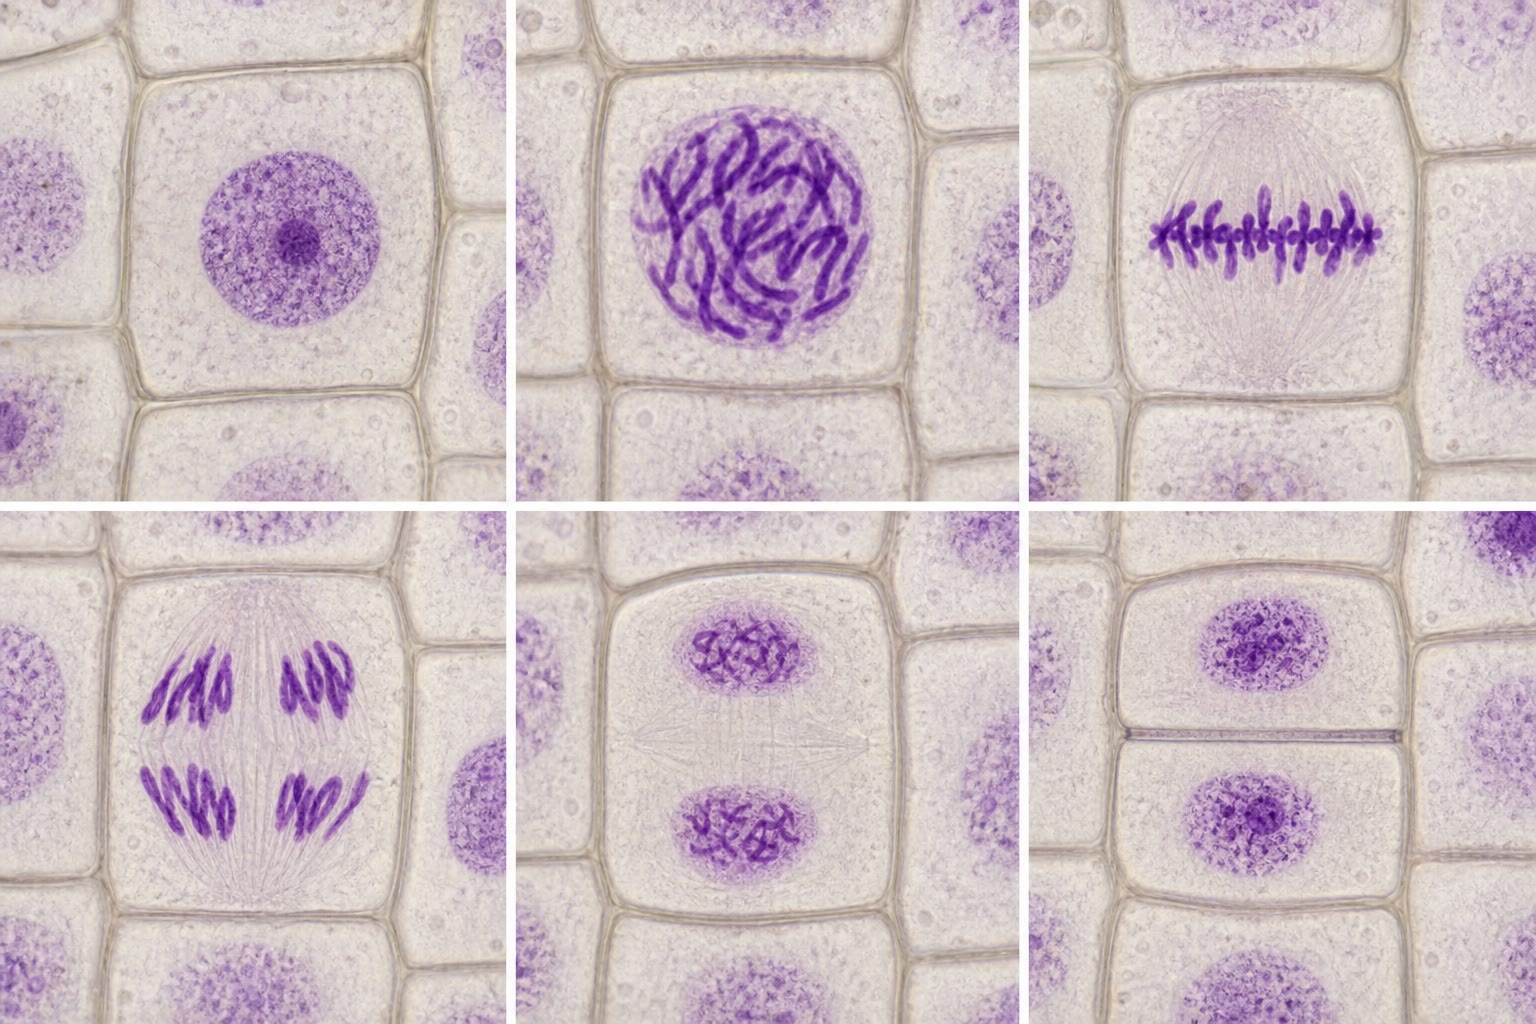
\includegraphics[width=0.9\linewidth]{images/book3/ai/b3-18-mitosis-grid.jpg}

{\small 洋葱根尖\omterm{def:b1:cell-unit-of-life:cell}{细胞}，分别处于\omterm{def:b1:replication-mitosis:cycle}{间期}、前期、中期、
后期、末期，以及胞质分裂之后，\omterm{def:b1:cell-unit-of-life:cell}{细胞}中部出现新的\omterm{def:b1:eukaryotic-cell:plantcell}{细胞壁}。
\omterm{def:b1:genomes:genome}{染色体}仅在凝缩时可见，自
前期至末期。}
\end{omfigure}

\begin{omfigure}
\begin{tikzpicture}[font=\footnotesize, >=Stealth, line cap=round]
  \foreach \i/\name in {0/前期, 1/中期, 2/后期, 3/末期} {
    \begin{scope}[xshift=\i*3.3cm]
      \draw[thick, omDef!70!black, fill=omDef!5] (0,0) ellipse (1.4 and 1.1);
      \node[anchor=north] at (0,-1.2) {\name};
    \end{scope}
  }
  % prophase: two centrosomes, condensed chromosomes (X shapes) scattered, envelope
  \begin{scope}
    \draw[thick, gray, dashed] (0,0) circle (0.8);
    \foreach \p/\a in {(-0.3,0.25)/30, (0.35,-0.1)/-40, (0.05,-0.45)/80} { \draw[very thick, omThm] \p ++(\a:0.22) -- ++(\a+180:0.44); \draw[very thick, omThm] \p ++(\a+60:0.22) -- ++(\a+240:0.44); }
    \fill[omProp!80!black] (-1.1,0.6) circle (0.07); \fill[omProp!80!black] (1.1,-0.6) circle (0.07);
    \foreach \a in {-30,0,30} { \draw[omProp!60!black] (-1.1,0.6) -- ++(\a-20:0.45); \draw[omProp!60!black] (1.1,-0.6) -- ++(\a+160:0.45); }
  \end{scope}
  % metaphase: spindle pole to pole, chromosomes on the plate
  \begin{scope}[xshift=3.3cm]
    \fill[omProp!80!black] (-1.25,0) circle (0.07); \fill[omProp!80!black] (1.25,0) circle (0.07);
    \foreach \y in {-0.5,-0.25,0,0.25,0.5} { \draw[omProp!60!black] (-1.25,0) -- (0,\y); \draw[omProp!60!black] (1.25,0) -- (0,\y); }
    \foreach \y in {-0.5,-0.17,0.17,0.5} { \draw[very thick, omThm] (-0.12,\y-0.14) -- (0.12,\y+0.14); \draw[very thick, omThm] (-0.12,\y+0.14) -- (0.12,\y-0.14); }
  \end{scope}
  % anaphase: chromatids moving to poles (V shapes)
  \begin{scope}[xshift=6.6cm]
    \fill[omProp!80!black] (-1.25,0) circle (0.07); \fill[omProp!80!black] (1.25,0) circle (0.07);
    \foreach \y in {-0.45,-0.15,0.15,0.45} { \draw[omProp!60!black] (-1.25,0) -- (-0.55,\y); \draw[omProp!60!black] (1.25,0) -- (0.55,\y); \draw[very thick, omThm] (-0.55,\y) -- (-0.35,\y+0.12) (-0.55,\y) -- (-0.35,\y-0.12); \draw[very thick, omThm] (0.55,\y) -- (0.35,\y+0.12) (0.55,\y) -- (0.35,\y-0.12); }
  \end{scope}
  % telophase: two nuclei reforming, cleavage furrow
  \begin{scope}[xshift=9.9cm]
    \draw[thick, gray, dashed] (-0.7,0) circle (0.45); \draw[thick, gray, dashed] (0.7,0) circle (0.45);
    \foreach \x in {-0.8,-0.6,0.6,0.8} { \draw[thick, omThm] (\x,-0.2) -- (\x,0.2); }
    \draw[very thick, omExo!70!black] (0,1.1) -- (0,0.55); \draw[very thick, omExo!70!black] (0,-1.1) -- (0,-0.55);
    \node[font=\scriptsize, omExo!70!black, anchor=south] at (0,1.15) {分裂沟};
  \end{scope}
\end{tikzpicture}

{\small 动物\omterm{def:b1:cell-unit-of-life:cell}{细胞}\omterm{def:b1:replication-mitosis:mitosis}{有丝分裂}的四个阶段。前期：
\omterm{def:b1:genomes:genome}{染色体}凝缩，\omterm{def:b1:replication-mitosis:mitosis}{纺锤体}由两个\omterm{def:b1:eukaryotic-cell:cytoskeleton}{中心体}形成。
中期：每条\omterm{def:b1:genomes:genome}{染色体}位于赤道面上，两侧分别与两极相连。
后期：姐妹\omterm{def:b1:replication-mitosis:mitosis}{染色单体}被拉开。末期：
两个\omterm{def:b1:eukaryotic-cell:nucleus}{细胞核}重新形成，分裂沟将\omterm{def:b1:cell-unit-of-life:cell}{细胞}一分为二。}
\end{omfigure}

\begin{omfigure}
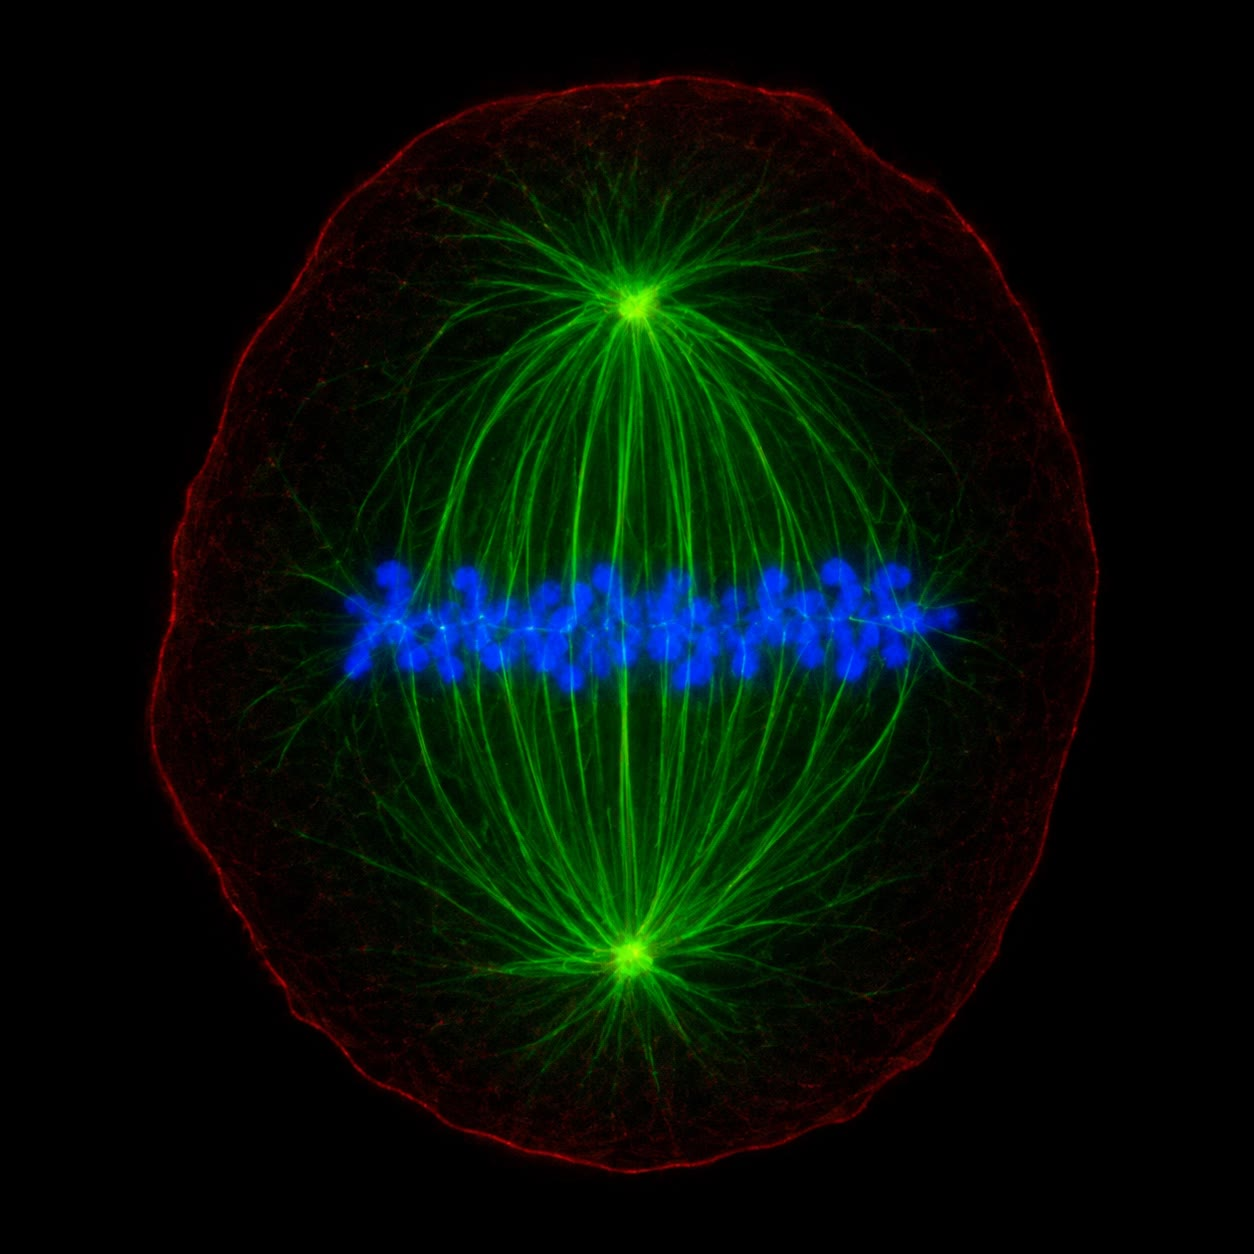
\includegraphics[width=0.4\linewidth]{images/book3/ai/b3-18-mitotic-spindle-fluorescence.jpg}

{\small 处于中期的培养\omterm{def:b1:cell-unit-of-life:cell}{细胞}，其\omterm{def:b1:eukaryotic-cell:cytoskeleton}{微管}以绿色标记，
\omterm{def:b1:genomes:genome}{染色体}以蓝色标记：\omterm{def:b1:replication-mitosis:mitosis}{纺锤体}横跨整个\omterm{def:b1:cell-unit-of-life:cell}{细胞}，从一极延伸至另一极，
\omterm{def:b1:genomes:genome}{染色体}在赤道面上排列成板状。}
\end{omfigure}

\begin{proposition}[有丝分裂所保持的量]\label{prop:b1:replication-mitosis:conserves}
\omterm{def:b1:replication-mitosis:mitosis}{有丝分裂}是保持\omterm{def:b1:genomes:genome}{染色体}数目的分裂：含 2n 条\omterm{def:b1:genomes:genome}{染色体}（人为 46 条）的\omterm{def:b1:cell-unit-of-life:cell}{细胞}
分裂为两个含 2n 条\omterm{def:b1:genomes:genome}{染色体}的\omterm{def:b1:cell-unit-of-life:cell}{细胞}。\omterm{def:b1:nucleic-acids:chain}{DNA}
含量由复制后的 $2q$ 降为每个子\omterm{def:b1:cell-unit-of-life:cell}{细胞}中的 $q$；
\omterm{def:b1:genomes:genome}{染色体}数目始终不变，因为\omterm{def:b1:genomes:genome}{染色体}以\omterm{def:b1:genomes:karyotype}{着丝粒}计数，
而每条\omterm{def:b1:replication-mitosis:mitosis}{染色单体}一旦分开，便成为一条\omterm{def:b1:genomes:genome}{染色体}。
由此，机体的每个\omterm{def:b1:cell-unit-of-life:cell}{细胞}在遗传上与其所来自的卵
完全相同，但复制时引入的突变除外。
使\omterm{def:b1:genomes:genome}{染色体}数目减半的分裂是减数分裂，
属于本科二年级分册。
\end{proposition}

\begin{method}[读取细胞周期实验]\label{met:b1:replication-mitosis:reading}
\begin{enumerate}
  \item 测量每个\omterm{def:b1:cell-unit-of-life:cell}{细胞}的 \omterm{def:b1:nucleic-acids:chain}{DNA} 含量（用一种荧光强度与 \omterm{def:b1:nucleic-acids:chain}{DNA} 含量
        成正比的染料，逐个\omterm{def:b1:cell-unit-of-life:cell}{细胞}测定）：含量为 $q$ 的\omterm{def:b1:cell-unit-of-life:cell}{细胞}处于 G$_1$ 期，
        含量为 $2q$ 的\omterm{def:b1:cell-unit-of-life:cell}{细胞}处于 G$_2$ 期或 M 期，介于两者之间的处于 S 期。
        各时期所占的\omterm{def:b1:cell-unit-of-life:cell}{细胞}比例即给出该时期的时长：某时期占整个周期的份额，
        就等于其\omterm{def:b1:cell-unit-of-life:cell}{细胞}所占的比例。
  \item 给予标记的\omterm{def:b1:nucleic-acids:nucleotide}{核苷酸}脉冲（溴脱氧尿苷）：仅处于 S 期的\omterm{def:b1:cell-unit-of-life:cell}{细胞}会摄入标记物；
        因此被标记\omterm{def:b1:cell-unit-of-life:cell}{细胞}的比例即为 S 期比例；
        追踪标记进入\omterm{def:b1:replication-mitosis:mitosis}{有丝分裂}的过程，便可得出
        G$_2$ 期的时长。
  \item 在染色切片中计数\omterm{def:b1:replication-mitosis:mitosis}{有丝分裂}图像：\emph{\omterm{def:b1:replication-mitosis:mitosis}{有丝分裂}
        指数}，即 M 期\omterm{def:b1:cell-unit-of-life:cell}{细胞}所占的比例，亦即 M 期占整个
        \omterm{def:b1:replication-mitosis:cycle}{细胞周期}的份额——对于 \qty{24}{h} 的周期、\omterm{def:b1:replication-mitosis:mitosis}{有丝分裂}
        历时一小时者，该值为 \qty{4}{\%}。
  \item 阻断某一步骤（能使\omterm{def:b1:eukaryotic-cell:cytoskeleton}{微管}解聚的药物可使\omterm{def:b1:cell-unit-of-life:cell}{细胞}停滞于
        中期，阻断 \omterm{def:b1:nucleic-acids:chain}{DNA} 合成的药物则使\omterm{def:b1:cell-unit-of-life:cell}{细胞}停滞于 S 期），
        然后统计积累起来的\omterm{def:b1:cell-unit-of-life:cell}{细胞}。
\end{enumerate}
\end{method}

\begin{example}[细胞更替]\label{ex:b1:replication-mitosis:turnover}
小肠\omterm{def:b1:body-plans-tissues:epithelium}{上皮}每四天更新一次，
皮肤每月更新一次，红\omterm{def:b1:cell-unit-of-life:cell}{细胞}每四个月从骨髓中补充一次，
骨髓每秒产生两百万个红\omterm{def:b1:cell-unit-of-life:cell}{细胞}；肝\omterm{def:b1:cell-unit-of-life:cell}{细胞}约每年分裂一次，
\omterm{def:b1:body-plans-tissues:nervous}{神经元}则几乎从不分裂。肿瘤\omterm{def:b1:cell-unit-of-life:cell}{细胞}已丧失了\omterm{prop:b1:replication-mitosis:checkpoints}{检查点}：
它们在不该分裂时仍然分裂，能耐受\omterm{def:b1:genomes:genome}{染色体}分离错误，
并积累使其分裂更快的突变。
化疗正是利用了这一差异：能毒害\omterm{def:b1:replication-mitosis:mitosis}{纺锤体}或
聚合酶的药物会杀死分裂最活跃的\omterm{def:b1:cell-unit-of-life:cell}{细胞}。
\end{example}

\section{练习}

\begin{exercise}[$\star$]\label{exo:b1:replication-mitosis:1}
解释为什么在\omterm{def:b1:replication-mitosis:fork}{复制叉}处，一条链是连续复制的，
另一条链则以片段的形式复制。
\end{exercise}

\begin{exercise}[$\star$]\label{exo:b1:replication-mitosis:2}
列出\omterm{def:b1:replication-mitosis:fork}{复制叉}处的酶和\omterm{def:b1:proteins:peptide}{蛋白质}及其
各自的作用。
\end{exercise}

\begin{exercise}[$\star$]\label{exo:b1:replication-mitosis:3}
由 \omterm{def:b1:nucleic-acids:chain}{DNA} 含量图读出 G$_1$ 期、G$_2$ 期及
\omterm{def:b1:replication-mitosis:mitosis}{有丝分裂}后的 \omterm{def:b1:nucleic-acids:chain}{DNA} 含量，以及各时期的\omterm{def:b1:genomes:genome}{染色体}数。
\end{exercise}

\begin{exercise}[$\star$]\label{exo:b1:replication-mitosis:4}
将\omterm{def:b1:replication-mitosis:mitosis}{有丝分裂}的各阶段排序，并给出每一阶段的标志性事件。
\end{exercise}

\begin{exercise}[$\star\star$]\label{exo:b1:replication-mitosis:5}
计算复制人类\omterm{def:b1:genomes:genome}{基因组}时产生的\omterm{def:b1:replication-mitosis:fork}{冈崎片段}数，
（\num{6.4e9} 个\omterm{thm:b1:nucleic-acids:helix}{碱基对}，片段长 \qty{150}{}），
以及由此所需的引物数、引物去除数和连接数。
\end{exercise}

\begin{exercise}[$\star\star$]\label{exo:b1:replication-mitosis:6}
计算人类\omterm{def:b1:genomes:genome}{基因组}每次复制的错误率：
仅聚合酶（$10^{-5}$）、带校对（$10^{-7}$）
及带错配修复（$10^{-9}$）时的情况，每次分裂
各产生多少个突变？
\end{exercise}

\begin{exercise}[$\star\star$]\label{exo:b1:replication-mitosis:7}
一个体\omterm{def:b1:cell-unit-of-life:cell}{细胞}每次分裂丢失 \qty{80}{} 个\omterm{def:b1:genomes:karyotype}{端粒}\omterm{def:b1:nucleic-acids:nucleotide}{核苷酸}，
起始\omterm{def:b1:genomes:karyotype}{端粒}长度为 \qty{10}{kb}，分裂至 \qty{5}{kb} 时停止，
该\omterm{def:b1:cell-unit-of-life:cell}{细胞}能分裂多少次？为什么癌\omterm{def:b1:cell-unit-of-life:cell}{细胞}需要\omterm{def:b1:genomes:karyotype}{端粒}酶？
\end{exercise}

\begin{exercise}[$\star\star$]\label{exo:b1:replication-mitosis:8}
某\omterm{def:b1:body-plans-tissues:tissue}{组织}中 \qty{5}{\%} 的\omterm{def:b1:cell-unit-of-life:cell}{细胞}处于\omterm{def:b1:replication-mitosis:mitosis}{有丝分裂}期，\qty{30}{\%} 处于
S 期；\omterm{def:b1:replication-mitosis:mitosis}{有丝分裂}持续一小时。计算\omterm{def:b1:replication-mitosis:cycle}{细胞周期}长度及
S 期的长度。
\end{exercise}

\begin{exercise}[$\star\star$]\label{exo:b1:replication-mitosis:9}
某\omterm{def:b1:cell-unit-of-life:cell}{细胞}的 2n $= 8$。给出其\omterm{def:b1:genomes:genome}{染色体}数、\omterm{def:b1:replication-mitosis:mitosis}{染色单体}数及
\omterm{def:b1:nucleic-acids:chain}{DNA} 含量（以 $q$ 计）在 G$_1$ 期、G$_2$ 期、中期，以及
末期后每个子\omterm{def:b1:cell-unit-of-life:cell}{细胞}的数目。
\end{exercise}

\begin{exercise}[$\star\star\star$]\label{exo:b1:replication-mitosis:10}
\emph{E. coli} 复制其\omterm{def:b1:genomes:genome}{染色体}需要 \qty{40}{min}，但
在营养丰富的培养基中每 \qty{20}{min} 分裂一次。解释其原因，并计算
\omterm{def:b1:cell-unit-of-life:cell}{细胞}在分裂时刻含有多少个复制起点和\omterm{def:b1:replication-mitosis:fork}{复制叉}。
\end{exercise}

\begin{exercise}[$\star\star\star$]\label{exo:b1:replication-mitosis:11}
秋水仙碱使\omterm{def:b1:eukaryotic-cell:cytoskeleton}{微管}解聚。预测用其处理的分裂\omterm{def:b1:cell-unit-of-life:cell}{细胞}会出现什么情况，
以及若其随后重新进入\omterm{def:b1:replication-mitosis:cycle}{间期}，\omterm{def:b1:genomes:genome}{染色体}数会如何变化，
并说明该药物为何用于制备\omterm{def:b1:genomes:karyotype}{核型}。
\end{exercise}

\begin{exercise}[$\star\star\star$]\label{exo:b1:replication-mitosis:12}
“\omterm{def:b1:replication-mitosis:mitosis}{有丝分裂}是先复制\omterm{def:b1:genomes:genome}{基因组}、再计数的过程。”请讨论：
用一段话说明复制保证了什么、\omterm{def:b1:replication-mitosis:mitosis}{纺锤体}保证了什么，
两者之间的\omterm{prop:b1:replication-mitosis:checkpoints}{检查点}的作用，以及在\omterm{def:b1:genomes:genome}{染色体}分离错误的\omterm{def:b1:cell-unit-of-life:cell}{细胞}中
什么环节会出现故障。
\end{exercise}

\section{问题：复制人类基因组}

\begin{problem}[{周末问题——S 期为八小时：复制叉计时、复制起点计数、
统计冈崎片段与引物，估算错误数，
并与细菌比较，最后得出复制起点的最少数目}]
\label{pb:b1:replication-mitosis:1}
人类\omterm{def:b1:cell-unit-of-life:cell}{细胞}在 S 期内复制 $\num{6.4e9}$ 个\omterm{thm:b1:nucleic-acids:helix}{碱基对}，该 S 期持续
\qty{8}{h}。真核生物\omterm{def:b1:replication-mitosis:fork}{复制叉}的移动速度为 \qty{50}{bp/s}；细菌
\omterm{def:b1:replication-mitosis:fork}{复制叉}为 \qty{1000}{bp/s}。\omterm{def:b1:replication-mitosis:fork}{冈崎片段}在真核生物中为 \qty{150}{}
个\omterm{def:b1:nucleic-acids:nucleotide}{核苷酸}，在细菌中为 \qty{1500}{} 个\omterm{def:b1:nucleic-acids:nucleotide}{核苷酸}。每添加一个
\omterm{def:b1:nucleic-acids:nucleotide}{核苷酸}需消耗两个 \omterm{def:b1:water-small-molecules:atp}{ATP} 当量（三磷酸前体）。单个碱基的错误率：
仅聚合酶为 $10^{-5}$，
带校对为 $10^{-7}$，带错配修复为 $10^{-9}$。

\medskip
\noindent\textbf{第一部分——\omterm{def:b1:replication-mitosis:fork}{复制叉}与复制起点。}
\begin{enumerate}
  \item 一个\omterm{def:b1:replication-mitosis:fork}{复制叉}在 \qty{8}{h} 内复制多少\omterm{thm:b1:nucleic-acids:helix}{碱基对}？
  \item 一个复制起点会发出两个\omterm{def:b1:replication-mitosis:fork}{复制叉}，一个复制起点
        在 \qty{8}{h} 内复制多少\omterm{thm:b1:nucleic-acids:helix}{碱基对}？
  \item 计算在 \qty{8}{h} 内复制完整\omterm{def:b1:genomes:genome}{基因组}所需的最少复制起点数，
        假定所有复制起点均在开始时启动。
  \item 计算这些复制起点沿 \omterm{def:b1:nucleic-acids:chain}{DNA} 的平均间距，分别以
        千碱基和微米为单位。
  \item 实际上，复制起点在整个 S 期陆续启动，约
        \num{40000} 个被使用。计算平均间距，以及
        一个\omterm{def:b1:replication-mitosis:fork}{复制叉}实际移动的平均距离。
  \item 最大的\omterm{def:b1:genomes:genome}{染色体}（\qty{250}{Mb}）若从其中心处的
        单个复制起点开始复制，需要多长时间？
  \item 解释为什么进化调整的是复制起点的数目、而非\omterm{def:b1:replication-mitosis:fork}{复制叉}的速度，
        以使 S 期变短。
\end{enumerate}

\medskip
\noindent\textbf{第二部分——片段与引物。}
\begin{enumerate}[resume]
  \item 计算一个 S 期内产生的\omterm{def:b1:replication-mitosis:fork}{冈崎片段}数。
  \item 计算铺设的 \omterm{def:b1:nucleic-acids:chain}{RNA} 引物数，包括
        每个复制起点处每条前导链上的一个引物。
  \item 计算所需的连接次数。
  \item 计算参与聚合反应的\omterm{def:b1:nucleic-acids:nucleotide}{核苷酸}总数（
        全\omterm{def:b1:genomes:genome}{基因组}两条链）。
  \item 计算聚合反应消耗的 \omterm{def:b1:water-small-molecules:atp}{ATP} 当量，以及
        整个 S 期内 \omterm{def:b1:water-small-molecules:atp}{ATP} 的平均消耗速率（每秒）。
  \item 与静息\omterm{def:b1:cell-unit-of-life:cell}{细胞}每秒约 $10^9$
        个 \omterm{def:b1:water-small-molecules:atp}{ATP} 的周转量相比较，该\omterm{def:b1:cell-unit-of-life:cell}{细胞}能量中有多大比例用于
        聚合反应？
\end{enumerate}

\medskip
\noindent\textbf{第三部分——错误。}
\begin{enumerate}[resume]
  \item 计算三种错误率下
        每个 S 期的错误数。
  \item 某\omterm{def:b1:genomes:gene}{基因}的编码序列为 \qty{1.5}{kb}。
        在完整的机制作用下，
        某一\omterm{def:b1:genomes:gene}{基因}在一次分裂中获得突变的概率为多少？
  \item 一个人的\omterm{def:b1:cell-unit-of-life:cell}{细胞}一生中约经历 $10^{16}$ 次分裂，
        在 $10^{-9}$ 的错误率下，总共会出现多少次突变？
        为什么机体能够耐受这一情况？
  \item 某次突变使错配修复失效。
        突变率将升高多少倍，
        这对一生中患癌症的风险有何影响？
\end{enumerate}

\medskip
\noindent\textbf{第四部分——细菌。}
\emph{E. coli}：\qty{4.6}{Mb}，一个复制起点，两个\omterm{def:b1:replication-mitosis:fork}{复制叉}。
\begin{enumerate}[resume]
  \item 计算复制整条\omterm{def:b1:genomes:genome}{染色体}所需的时间。
  \item 在营养丰富的培养基中，\omterm{def:b1:cell-unit-of-life:cell}{细胞}每 \qty{20}{min} 分裂一次。
        同时有多少轮复制在进行，
        新生\omterm{def:b1:cell-unit-of-life:cell}{细胞}带有多少个复制起点？
  \item 计算每轮复制产生的\omterm{def:b1:replication-mitosis:fork}{冈崎片段}数，
        以及每秒产生的\omterm{def:b1:replication-mitosis:fork}{冈崎片段}数。
  \item 计算在 $10^{-9}$ 错误率下每轮复制的错误数，
        以及带有新突变的子\omterm{def:b1:cell-unit-of-life:cell}{细胞}所占的比例。
  \item 一个每毫升含 $10^9$ 个\omterm{def:b1:cell-unit-of-life:cell}{细胞}的培养物分裂一次，
        每毫升会出现多少个新突变，
        其中有多少个落在某个 \qty{1}{kb} 的特定\omterm{def:b1:genomes:gene}{基因}上？
  \item 解释为什么几乎任何大规模的敏感菌株培养物中，
        都会出现抗生素抗性。
  \item 比较两种生物：\omterm{thm:b1:nucleic-acids:helix}{碱基对}数、复制起点、
        \omterm{def:b1:replication-mitosis:fork}{复制叉}速度、S 期时长，
        以及使更大的\omterm{def:b1:genomes:genome}{基因组}能在相近时间内完成复制的设计。
  \item 给出结论：人类 S 期为 \qty{8}{h} 时，所需的最少复制起点数，
        以及实际的数目和间距。
\end{enumerate}
\end{problem}
